\section{Videnssamling}
\begin{frame}{Videnssamling}
Vi forsøgte at gøre brug af forskellige teknikker til videnssamling igennem iterationerne:
\begin{enumerate}
\item Interview med administratorer og state of the art
\item Interview med gæster
\item Vertikal prototype med Fabrikken
\item Usability test på en mobil enhed
\end{enumerate}
\end{frame}

\subsection{State of the Art}
\begin{frame}{State of the Art}
	Nogle af de koncepter vi fandt fra eksisterende systemer:
	Playliste, afstemme og anmode
	\begin{itemize}
	\item Vægtet - SecretDJ og Rockbot
	\item Begrænset - SecretDJ
	\item Stemme ned og indirekte anmodning - Mixgar
	\end{itemize}

	Resultat: Ideer til koncepter der kan bruges bruges i netop denne kontekst.
\end{frame}
\subsection{Interviews og informanter}
\begin{frame}{Interviews og informanter}
	Semi-strukturede interviews, for bl.a. at kunne grave ned i de eksisterende løsningers problemmer.

	To grupper af aktører:
	\begin{itemize}
		\item Dem der råder over musikken, administratorne.
		\item Dem der lytter til musikken i konteksten, gæsterne.
	\end{itemize}

	Kontekstuelle interviews
	
	Resultat: En bedre forståelse for konteksten og krav til systemet, fra begge aktørers side.
\end{frame}
\subsection{Prototyper}
\begin{frame}{Prototyper}
	\begin{multicols}{2}
		\begin{figure}
			\centering
			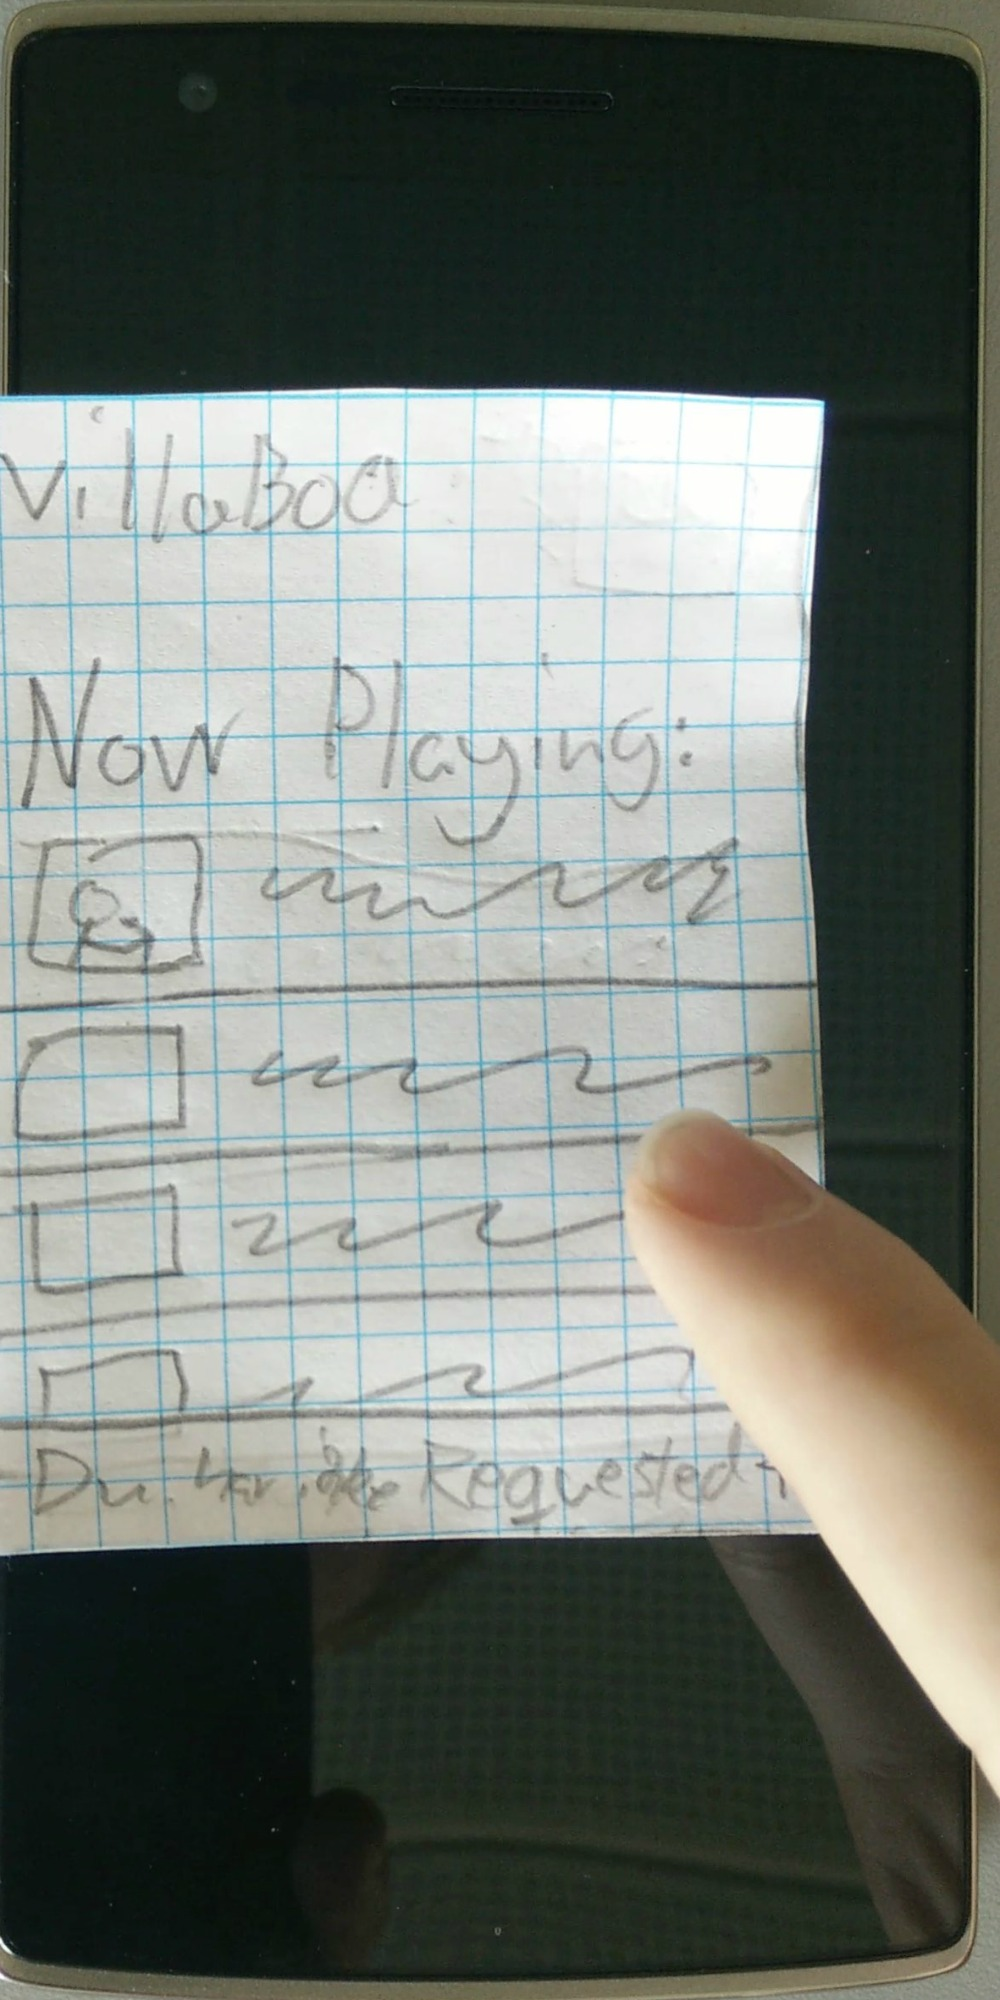
\includegraphics[height=\textwidth/3]{slides/Heider/paperPrototypeVoteInteraction}
			\caption{Papirprototype}
		\end{figure}
		\columnbreak
		\begin{figure}
			\centering
			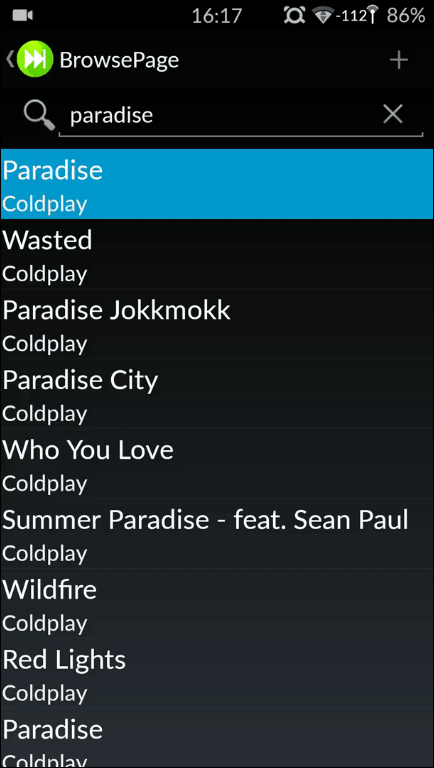
\includegraphics[height=\textwidth/3]{slides/Heider/search}
			\caption{Vertikal}
		\end{figure}
	\end{multicols}
	\begin{itemize}
	\item Udforskende papirprototyper i design fasen til at afprøve nye ideer til design.
	\item Vertical vurderende prototyper til valg af design og skabelse af nye krav.
	\end{itemize}
\end{frame}
\subsection{Usability test}
\begin{frame}{Usability test}
	\begin{multicols}{2}
		\begin{figure}
			\centering
			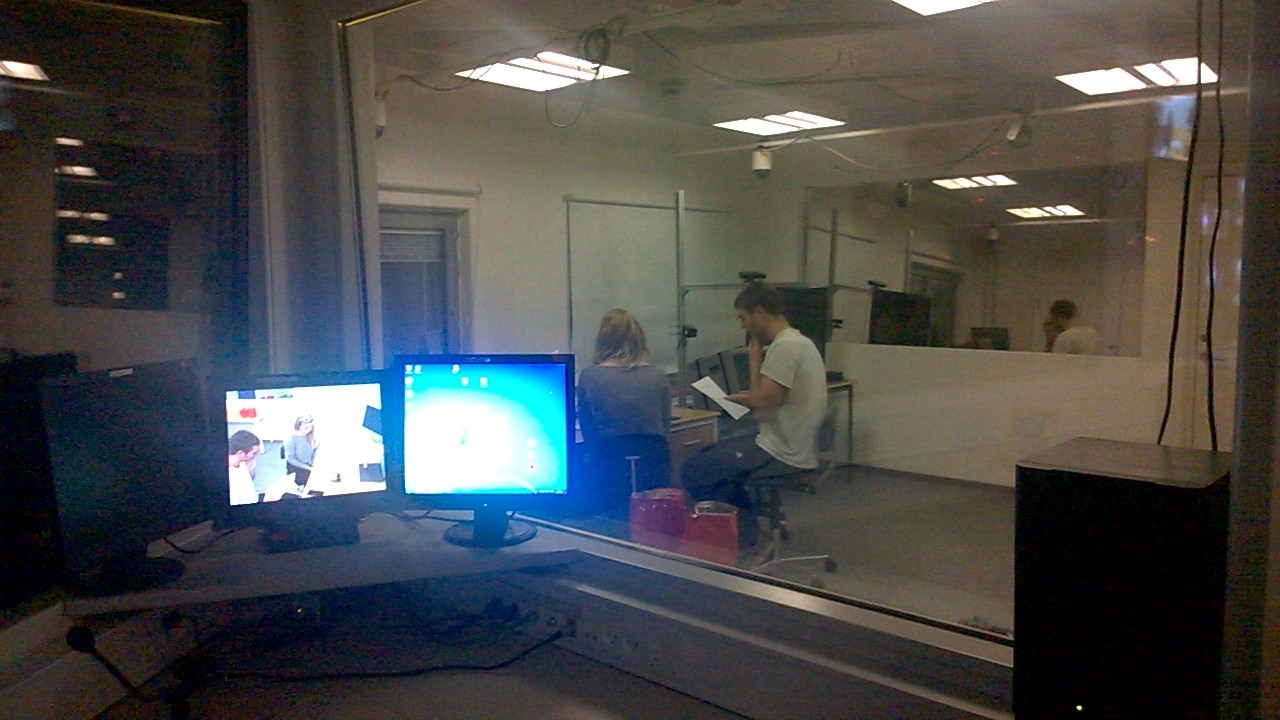
\includegraphics[width=\textwidth/2]{slides/Heider/subjectRoom}
		\end{figure}
		\columnbreak
		Vi forberedte nogle opgaver som brugerne skulle igennem.
		Roller:
		\begin{itemize}
			\item Dataloggere
			\item Testleder
			\item Videooperatør
			\item Simulator af social interaktion
			\item Transport og forberedelse af testpersoner
		\end{itemize}
	\end{multicols}
	Til analyse brugte vi Instant Data Analysis, da det er hurtigt og finder næsten alle de samme problemmer som traditionel video analyse.

	Resultat: Indsigt i nogle problemmer med det valgte design og nye krav.
\end{frame}
